\section{Preliminaries} 
\label{sec:Prelim} 

Our work and contribution relies mainly on three structures, a \textit{monoid}, a \textit{set} and a \textit{finger tree}, which are briefly described in the following subsections. 

\subsection{Monoid}

A \textit{monoid} is a triple $(S,\star,e)$, where $S$ is a set, $\star$ is a binary operation, called $product$ and $e$ is an element of $S$, called $unit$, satisfying the following properties:

\begin{enumerate}
\item $e \star x = x = x \star e$, for all $x \in S$ 
\item $x \star (y \star z) = (x \star y) \star z $, for all $x,y,z \in S$.  
\end{enumerate}

As an example of a Haskell implementation of a monoid we have:
%\begin{verbatim}
\begin{lstlisting}[mathescape]
class Monoid  a where 
   mempty  :: a
   mappend :: a $\to$ a $\to$ a
\end{lstlisting}   
%\end{verbatim}

where the function \code{mempty} represents the element $e$ and the function \code{mappend} represents function $\star$. Detailed information about monoids within the functional programming can be found in \cite{Monoids}, and for the Haskell implementation at \cite{HaskellMonoid}.


\subsection{Set as binary search tree}
A \textit{binary search} tree (BST) is either a \textit{leaf} (also called a \code{tip}) or a vertex consisting of a \textit{value}, a \textit{left} BST and a \textit{right} BST. The height of the tree determines the time taken to perform every operation onto it, therefore the shorter the height the better, and this is done throughout a \textit{balancing scheme}. The study of BSTs is vast and there are several implementation around. In our case, a \textit{size balanced} is used. A detailed comparison and benchmarking is outside the scope of the present work.

\tcr{My main criticism of the paper is the presentation. While I appreciate the use of diagrams in the first half of the paper, high-level explanations are missing later. The paper does not do a very good job providing an intuition for how the data structure works. For example, I was struggling understanding the role of the monoidal set. The paper also explains too little of the background regarding used existing data structures and their realisation in Haskell libraries. For example, the interface to the finger tree ADT and the Measured type class. In general, most of the explanations are closely tight to the code but don’t give a high-level picture of what individual operations do in terms of the Euler tour. Given that there is plenty of space left in the paper, this could be improved in the final version.}


The following is an snippet of \code{Data.Set} \footnote{https://hackage.haskell.org/package/containers-0.5.10.2/docs/Data-Set.html}
%\begin{verbatim}
\begin{lstlisting}
data Set a    = Bin Size a (Set a) (Set a)
              | Tip
\end{lstlisting}              
%\end{verbatim}

In Table~\ref{tab:Setfuncs} we show the set-functions we have incorporated in \code{dynTsET} from \code{Data.Set}.
\small
\begin{table}
\begin{center}
\begin{tabular}{||l | l | c||} 
 \hline
 Function         & Type                                   & Time complexity            \\ 
 \hline\hline
 \texttt{empty}   & \texttt{Set a}                         & $O(1)$                     \\ 
 \hline
 \texttt{insert}  & \texttt{a $\to$ Set a $\to$ Set a}     & $O(\log n)$                \\
 \hline
 \texttt{member}  & \texttt{a $\to$ Set a $\to$ Bool}      & $O(\log n)$                \\ 
 \hline
 \texttt{union}   & \texttt{Set a $\to$ Set a $\to$ Set a} & $O(m(\log\frac{n}{m} +1))$ \\
 \hline
\end{tabular}
\caption{Leijen's implementation of \code{Data.Set} \cite{HaskellSet}, based on \cite{ParallelSets}}
\label{tab:Setfuncs} 
\end{center}
\end{table}
\normalsize

Functions \code{empty} and \code{union} are, in fact, the monoidal functions \code{mempty} and \code{mappend} respectively. 

\subsection{Euler-tour tree} 

Dealing with trees of different degree can be complicated. A simple way to handle and represent trees of any degree is by an Euler tour, that is, a sequence as in \cite{Rand-DynGs-Algos} and \cite{WerneckR-PhD}. To represent a tree $t$, we replace every edge $\langle u,v \rangle$ of $t$ by two arcs $(u,v)$ and $(v,u)$, and add a loop $(v,v)$ to represent each vertex $v$. In this context, a tree $t$ can have at least one, and in general, many Euler tours. The size of an Euler tour \textit{et} of $t$ is $et(t) = v + 2e $, where $v$ is the number of vertices of $t$ and $e$ its number of edges. We can represent an Euler tour in Haskell simply as a list of pairs, such in 

%\begin{verbatim}
\begin{lstlisting}
data EulerTour a = [(a,a)] 
\end{lstlisting}
%\end{verbatim}

By managing the tour with lists, we can perform insertion from the left (head) in $O(1)$ but remaining operations such insertion from the right, access, cutting, appending and inserting might take $O(n)$ per operation.
On the other hand, representing tours through finger trees, performance per operation is improved up to $O(\log n)$ per operation amortised as we explain shortly and in Section~\ref{sec:TechDes}. 

Our representation of $k$-trees through Euler-tour will not close up the tour with the first node as this avoids the uniqueness presence for such a node, as shown in Fig.~\ref{fig:Euler-tour}.

\begin{figure}
\begin{center}
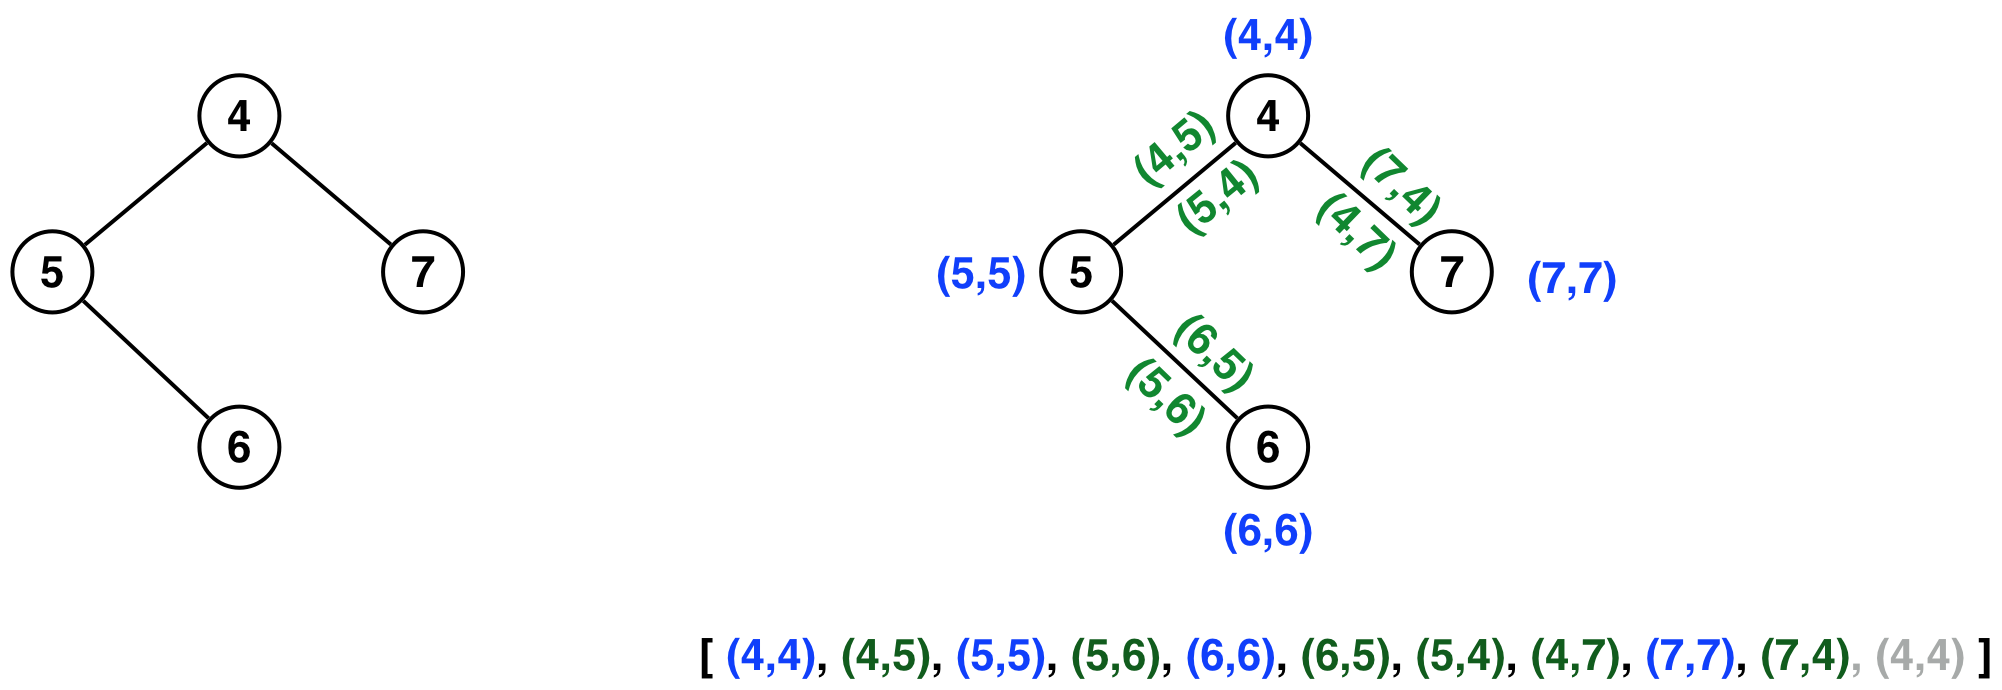
\includegraphics[scale=0.35]{./Images/Euler-tour} 
\end{center}
\caption{The $k$-tree (left) is represented as a sequence of size $v+2e$ (right). Notice we left out the final node-pair to preserve uniqueness}
\label{fig:Euler-tour}
\end{figure}



\subsection{Finger tree} 

We present Hinze and Paterson's version of finger trees \madd{(FTs)} \cite{FTs}, followed by the functions we have used for the \code{dynTsET}.

\begin{figure}
\begin{lstlisting}
data FingerTree v a = Empty
                    | Single a 
                    | Deep v 
                           Digit a 
                           FingerTree v (Node v a) 
                           Digit a
\end{lstlisting}                           
\caption{Data type of the finger tree by Hinze and Ross}
\label{fig:FTdatatype}
\end{figure}

\tcr{This reviewer can't help but think that there seems to be a lot of redundancy in the proposed data structure, as the Euler tour node pairs are present in both the sets and in the finger trees.}


\code{Digit} type holds from one up to four elements of type \code{a}. \code{Node} type can hold two or three elements of type \code{a}. The recursive and nested definition of \code{FingerTree} forces the structure to be balanced by its types, instead of enforcing it by code invariants. Finger trees are 2-3 trees where values are stored at the leaves, in our case those leaves are the pairs representing an Euler tour. To implement \textit{updates} and \textit{lookups} efficiently, Hinze and Paterson \cite{FTs} added a monoidal annotation on the intermediate vertices, the \code {v} type.

In figure Fig.~\ref{fig:FT-Euler-tour} we can see our example of the Euler-tour sequence in Fig.~\ref{fig:Euler-tour} managed by the data constructors described above.

\begin{figure}
\begin{center}
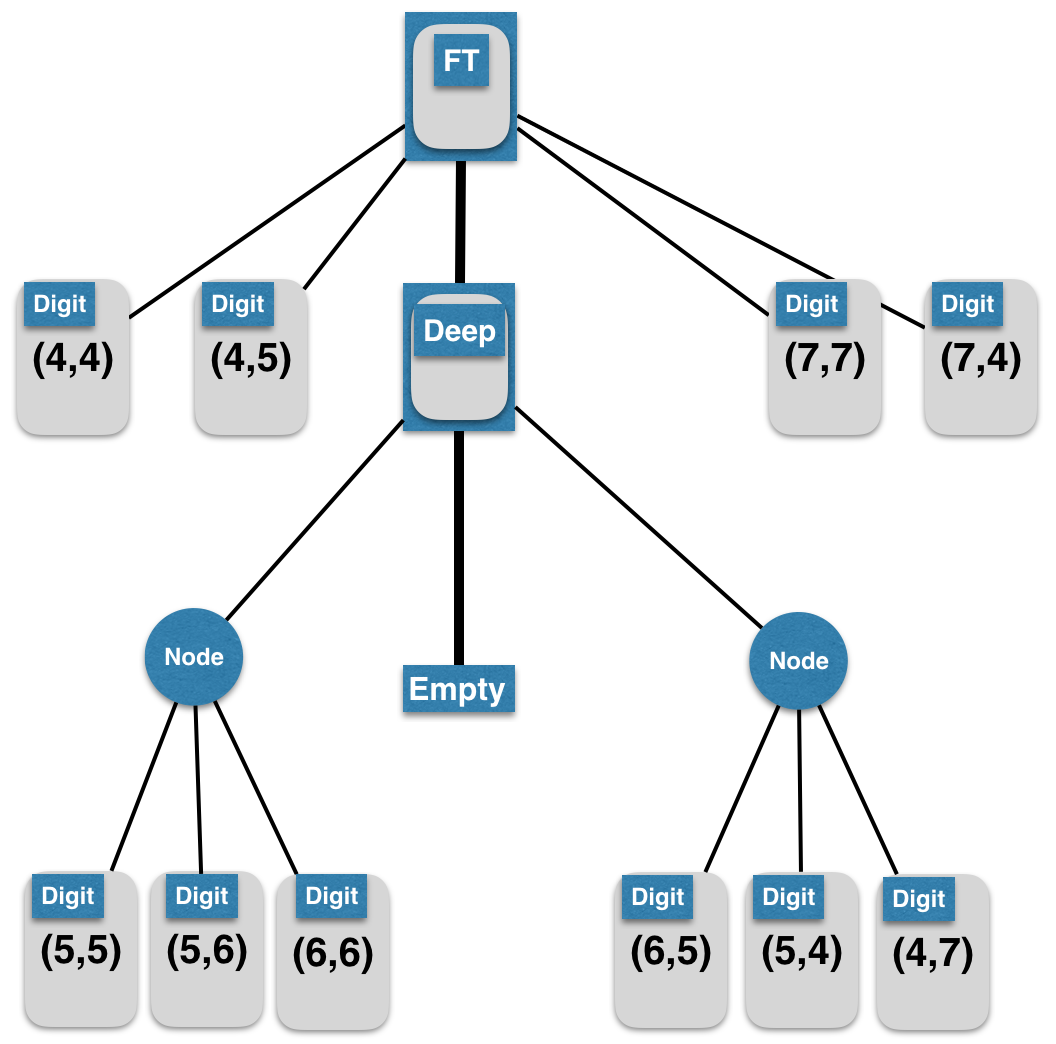
\includegraphics[scale=0.35]{./Images/FT-Euler-tour} 
\end{center}
\caption{A finger tree (FT) holding the sequence (Euler-tour) that represents the $k$-tree in Fig.\ref{fig:Euler-tour}}
\label{fig:FT-Euler-tour}
\end{figure}




\tcb{SPLIT is not longer used, instead there is SEARCHFT, which aim is the same as SPLIT and hope it will be easier to explain}

\tcb{Is it the ``best" part in the document to bring up an explanations or examples or both for amortisation?}